%!TEX root = thesis.tex
\section{Concept}
\section{Related work and approaches}
\subsection{Electronic Textiles}
\begin{quotation}
\emph{The most profound technologies are those that disappear. They weave themselves into the fabric of everyday life until they are indistinguishable from it. \citep{weiser1991computer}}
\end{quotation}
One of the research areas that have stemmed from ubiquitous computing is electronic textiles or `e-textiles', which seeks to integrate electronic and computation into fabric.
\citet{park2002wearable} presents the E-Textile vision as the paradigm the ``fabric is the computer'', taking Weiser's much quoted description of ubiquitous computing very literal.
One of the main obstacles for attaining this vision of the \emph{fabric as the computer} is how to incorporate the underlying computation into the fabric.
There are generally seen three ways to do it, either by computing \emph{offline}, on a separate system connected to the fabric, \emph{onto}, on components attached to the fabric or \emph{into} the fabric, embedded seamlessly into it \citep{marculescu2003}.
Today computation is commonly done either offline or onto the fabric, or a combination of the two, but advances in organic electronics and nano technology, for example with organic transistors weaved into fabric \citep{lee2005weave}, suggests that computation embedded into the fabric is not far off.
\begin{figure}
\centering
\begin{minipage}[t]{.3\textwidth}
  \centering
  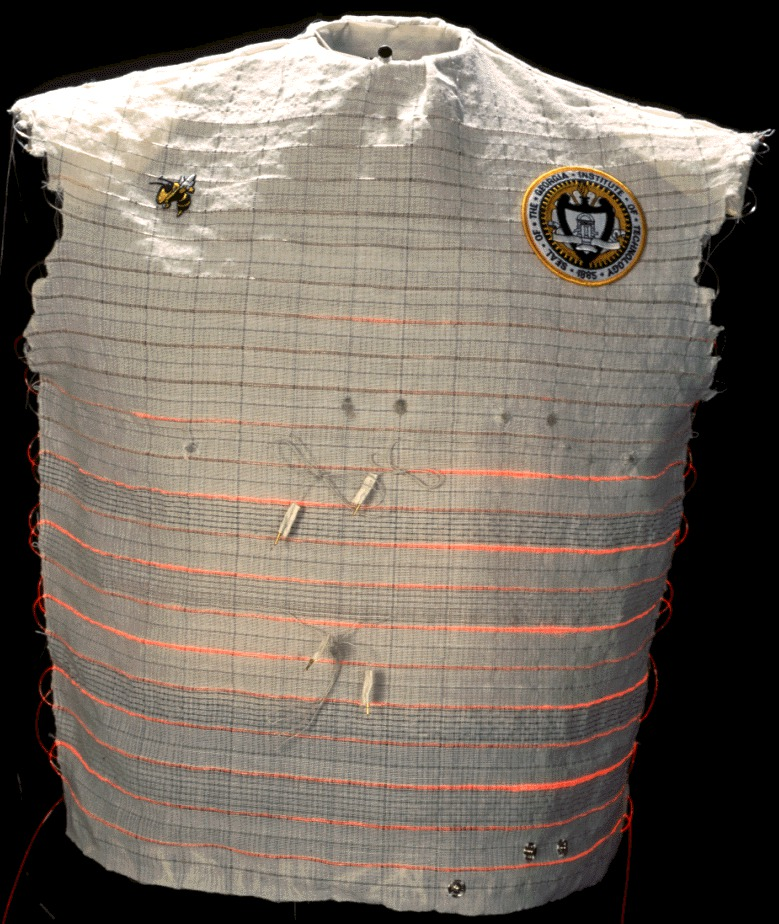
\includegraphics[width=0.8\linewidth]{figures/wearable_motherboard}
  \captionof{figure}{The Wearable Motherboard, taken from \citep{gopalsamy1999wearable}}
  \label{sofa_interaction:wearable_motherboard}
\end{minipage}%
\hspace{0.2cm}
\begin{minipage}[t]{.3\textwidth}
  \centering
  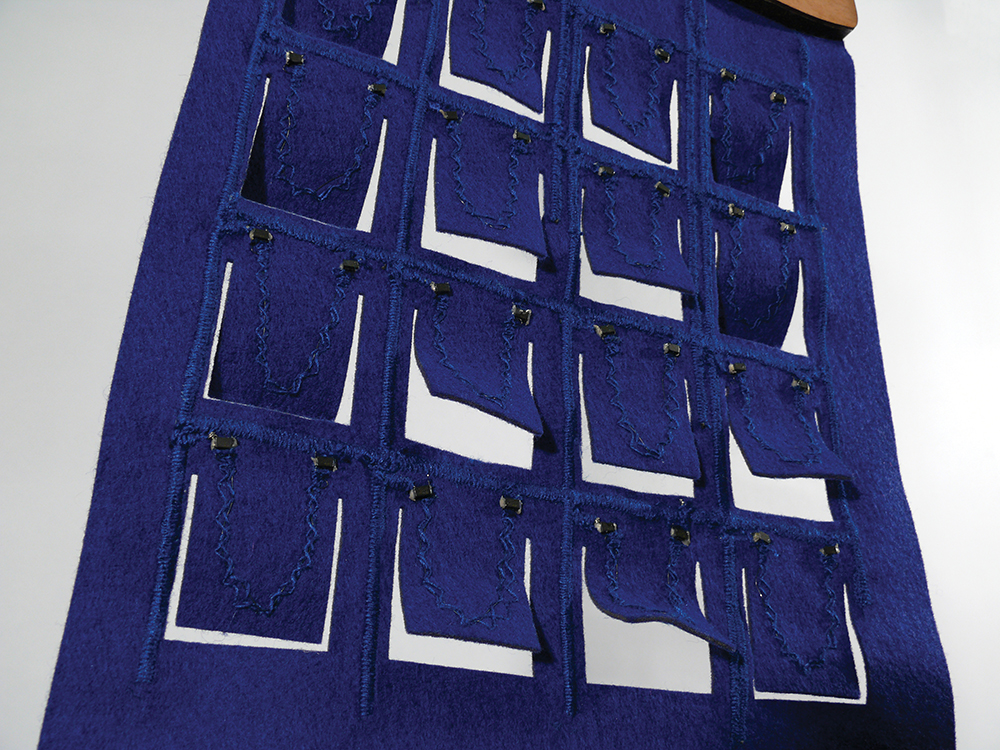
\includegraphics[width=0.8\linewidth]{figures/shutters}
  \captionof{figure}{Shutters, taken from \citep{coelho2009shutters}}
  \label{sofa_interaction:shutters}
\end{minipage}
\hspace{0.2cm}
\begin{minipage}[t]{.3\textwidth}
  \centering
  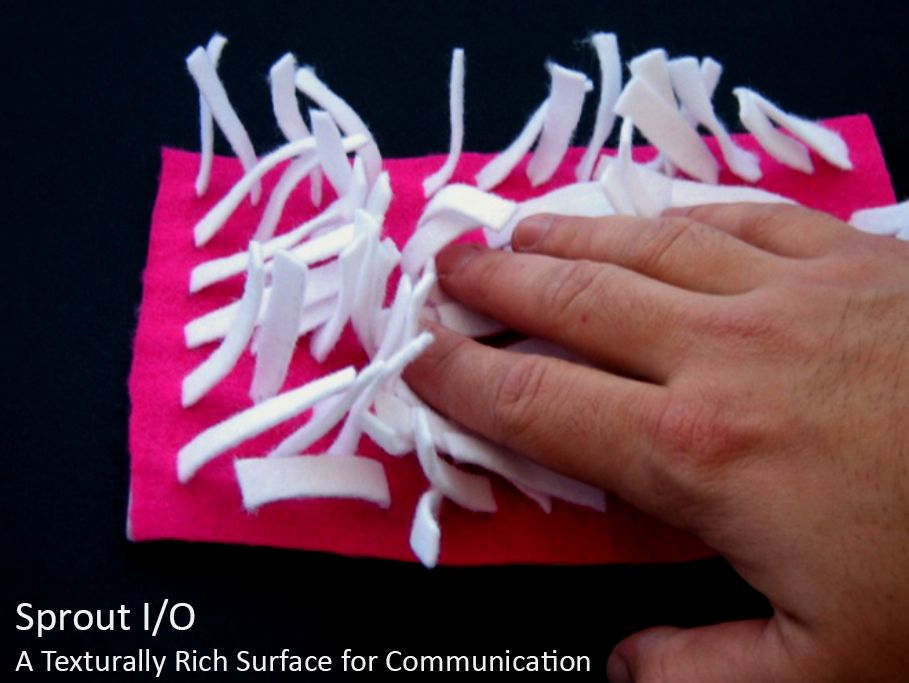
\includegraphics[width=0.8\linewidth]{figures/sprout}
  \captionof{figure}{Sprout I/O, taken from \citep{coelho2009shutters}}
  \label{sofa_interaction:sprout}
\end{minipage}
\end{figure}
E-textile is often seen used as part of wearable computing systems, logically, since clothing as a medium is ever present when people are involved.
An example of this is the Wearable Motherboard \citep{gopalsamy1999wearable} seen in figure~\ref{sofa_interaction:wearable_motherboard}, also called the ``Smart Shirt'', which is a lightweight monitoring `shirt' that can provide sensory data for use in medical and military contexts.
The fabric here is used as data paths that facilitates routing of information from any point to any other point on the shirt through conductive fibers embedded in the fabric.

E-textiles are not limited to wearable computing and clothing, and can just as well be part of interior design such as curtains, pillows, carpets, upholstery ect.
Shutters by \citet{coelho2009shutters}, seen in figure~\ref{sofa_interaction:shutters}, is an example of this where shape-memory alloy (SMA) threads are woven into a felt surface creating a curtain-like structure capable change of shape in permeability, used for indoor ventilation control among other things.
Here the SMA allows for actuation in the shutters while retaining the look, feel and softness of textile without any hard mechanic actuators.  
Another example from \citet{coelho2008sprout} is Sprout I/O, see figure~\ref{sofa_interaction:sprout}, where a membrane filled with strands of SMA and felt provides textually rich input and actuated output capabilities.
By measuring the capacitance between the users hand and the SMA threads touches can be registered, enabling stroke-like interaction, by creating an input matrix that register changes in each of the the individual SMA threads.

We have gotten a lot of inspiration from the various ``Do It Yourself'' (DIY) on-line communities related to e-textile craft and crafts in general, notably KOBAKANT DIY \citep{kobakantWEB} and Instructable \citep{instrucableWEB}.
Both sites provides guides, tips, and tricks for materials, construction and techniques and have for us been a good starting point for doing an e-textile project.
One of our inspirations has been rSkin \citep{rskinplusea,rSsininstructables}, a project by Hannah Perner-Wilson, which attempts to create a `skin' for a robot arm, made out of textiles, that enables the arm to register intensity and location of touches on the whole arm, seen in figure~\ref{rskin}.

\begin{figure}[hb]
	\centering
  		\includegraphics[width=3in]{figures/rskin}
	\caption[rSkin, Open Source Robot Skin]
   {rSkin, Open Source Robot Skin}
   \label{rskin}
\end{figure}

The `skin' is made of stretchy fabric and a 28 rows x 28 columns large pressure sensitive grid is embedded into the fabric using conductive thread.
The skin is made out of three layers: first a non-conductive layer with 28 rows of conductive thread, then a layer piezoresistive fabric and lastly a non-conductive layer with 28 columns of conductive thread.
The piezoresistive fabric acts as a pressure sensitive layer as piezoresistive materials decrease their electrical resistivity under mechanical stress \citep{piezoresistiveWIKIPEDIA}.
This approach to making pressure sensitive grids will be described in further detail in the next section as we build upon it, in our own prototype.

\subsection{Touch Sensing}
Generally seen there are three broad categories for doing multi-touch input sensing: optical, capacitive and resistive \citep{rosenberg2009unmousepad}.

Optical sensing usually involve one or more digital cameras placed behind the touch surface to generate an image of the user's finger to track the interaction.
As this approach relies on cameras it is typically used for larger applications such as tabletops, e.g. reacTable \citep{jorda2007reactable} and the tabletop version of Microsoft Surface.

Capacitive sensing systems for touch based interaction rely on the human body's capacitive abilities to acquire the position of the touch on a surface. 
As a finger touches the surface, the surface's electrostatic field distorts and this change is then measurable as a change in capacitance at some position in a 2d grid.
The most common example of this approach is the touch surface of modern smart phones and tablets where touch has become the preferred form of interaction.
Another example is Touch\'e \citep{sato2012touche} that allow objects and environments to become touch sensitive, allowing everyday objects to become touch interfaces, such as doorhandles, cups, water bottles ect.
This is done by sending a signal through the object and doing electromagnetic frequency sweeps. 
These frequencies will change when a touch occur and will change based on the size of the touched on the surface allowing for simple gesture recognition.
Two limitations of this technology is that pressure can not reliably be measured and that most systems based this technology only works with bare skin touching it.    

Resistive sensing
\section{Technicalities}
\section{Evaluation}